% 01-prologue/slides.tex, v. 1 (21/12/12)
% companion files to "Language and Computers"
% Dickinson, Brew, & Meurers (2013)

\documentclass{beamer}

\usepackage{graphicx}
\usepackage{forest,adjustbox}
\useforestlibrary{linguistics}
\forestapplylibrarydefaults{linguistics}
\usepackage{mrs}
\usepackage{avm}

\title{Introduction to NLP}
\subtitle{Syntax and Parsing. Context Free Grammars}
\author{Alexandre Rademaker \thanks{Olga Zamaraeva}}
\institute{FGV/EMAp}


\begin{document}
   
\begin{frame}
  \maketitle
\end{frame}

\section{Overview}

\begin{frame}{Overview}
  \begin{itemize}
  \item Parsing: constituent and dependency
  \item Leonard Bernstein's musical syntax
    \begin{itemize}
    \item \url{https://www.youtube.com/watch?v=r_fxB6yrDVo}
    \end{itemize}
  \item Target representations
  \item Context Free Grammars
  \item Evaluating parsing
  \item Treebanking
  \end{itemize}
\end{frame}

\section{Parsing}

\begin{frame}{Parsing}
  \begin{itemize}
  \item Recognizing string as input and assigning structure to it
  \item Syntactic parsing: assigning syntactic structure
  \item Semantic parsing: assigning semantic structure
  \end{itemize}
\end{frame}

\begin{frame}{Syntactic Parsing}

  Parsing: Making explicit structure that is inherent (implicit) in
  natural language strings

\begin{itemize}
\item What is that structure?
\item Why would we need it?
\end{itemize}

\vspace{.5cm}

\begin{columns}\tiny
  \begin{column}{0.5\textwidth}
    \begin{forest}
      [S
       [NP 
         [I]]
       [VP
        [saw]
        [NP [the] [astronomer]
          [PP [with the telescope,roof]]]
       ]
      ]
    \end{forest}
  \end{column}
  \begin{column}{0.5\textwidth}
    \begin{forest}
	[S
		[NP 
            [I ]]
		[VP
			[saw]
			[NP [the] [astronomer]]
			[PP [with the telescope,roof]]
		]
	]
      \end{forest}
    \end{column}
  \end{columns}
\end{frame}

\begin{frame}{Parsing}

  Parsing: Making explicit structure that is inherent (implicit) in
  natural language strings

  \begin{itemize}
  \item What is that structure?
  \item Why would we need it?
  \end{itemize}

  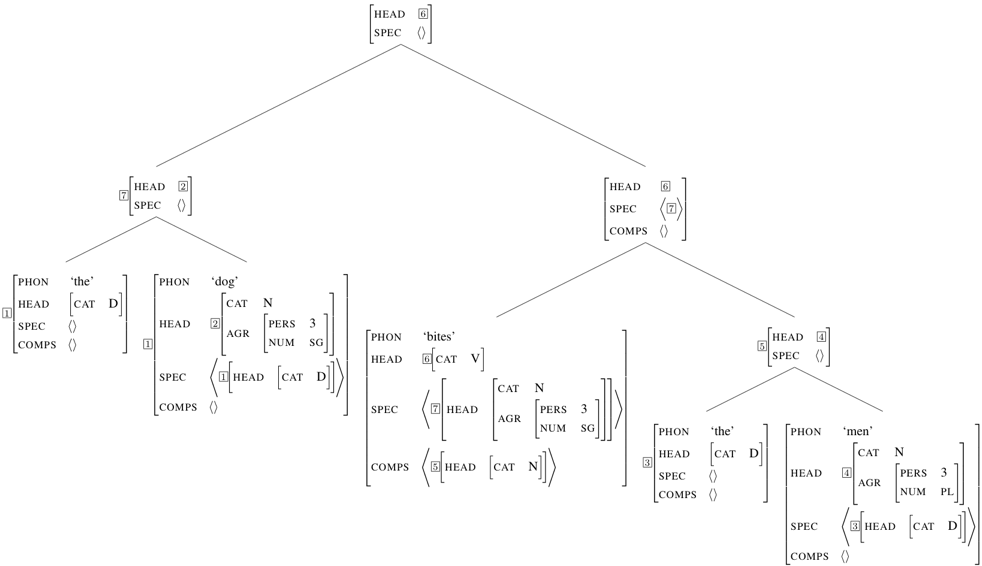
\includegraphics[height=0.55\textheight]{figures/hpsg1}

  {\tiny pic from:
    \url{http://www.dobnik.net/simon/teaching/shared/LT2112-formling/pics/?MA}}
\end{frame}

\begin{frame}{Implicit structure}
  \begin{itemize}
  \item What do these sentences have in common?
    \begin{itemize}
    \item Kim gave the book to Sandy.
    \item Kim gave Sandy the book.
    \item The book was given to Sandy by Kim.
    \item This is the book that Kim gave to Sandy.
    \item Which book did Kim give to Sandy?
    \item Kim will be expected to continue to try to give the book to Sandy.
    \item This book everyone agrees Pat thinks Kim gave to Sandy.
    \item This book is difficult for Kim to give to Sandy.
    \end{itemize}
  \end{itemize}
\end{frame}

\begin{frame}{Implicit structure: Constituent structure \& Dependency structure}
\small
 Kim gave the book to Sandy.
 \begin{itemize}
 \item (S (NP Kim) (VP (V gave) (NP (D the) (N book)) (PP (P to) (NP Sandy))))
 \item subj(gave, Kim); dobj(gave, book); iobj(gave, to); dobj(to, Sandy); spec(book, the)
 \end{itemize}

 \begin{columns}
   \begin{column}{0.5\textwidth}
     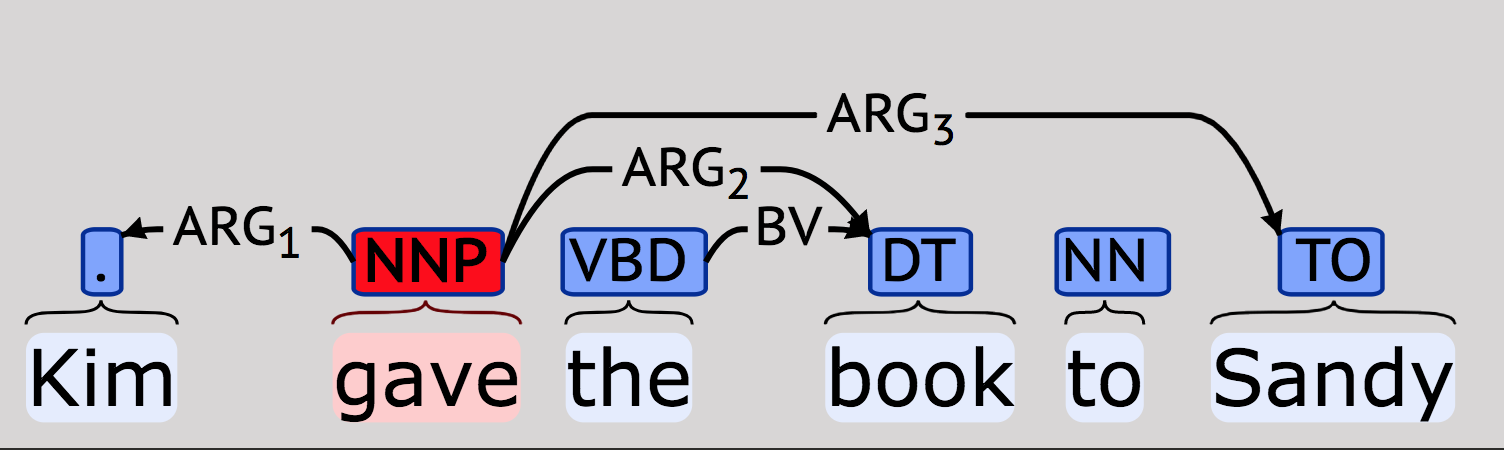
\includegraphics[width=\textwidth]{figures/depend1}      
   \end{column}
   \begin{column}{0.5\textwidth}
     \begin{forest}
       [S
        [NP [Kim]]
        [VP [V [gave]] [NP [D[the]] [N[book]]] [PP [P [to]] [NP [Sandy]]]]
       ]
     \end{forest} 
   \end{column}
 \end{columns}
\end{frame}

\begin{frame}{Dependency parsing}

  \begin{itemize}
  \item Instead of constituents, look at grammatical relations between heads of constituents
    \begin{itemize}
    \item Why?
    \end{itemize}
  \item flexible word order
  \item semantics
  \item relations between active and passive
  \item Harder to explain the {\bf ungrammaticality} of certain constructions
    \begin{itemize}
    \item lack of theoretical ground
    \end{itemize}
  \end{itemize}
\end{frame}

\begin{frame}{Dependency structure}
  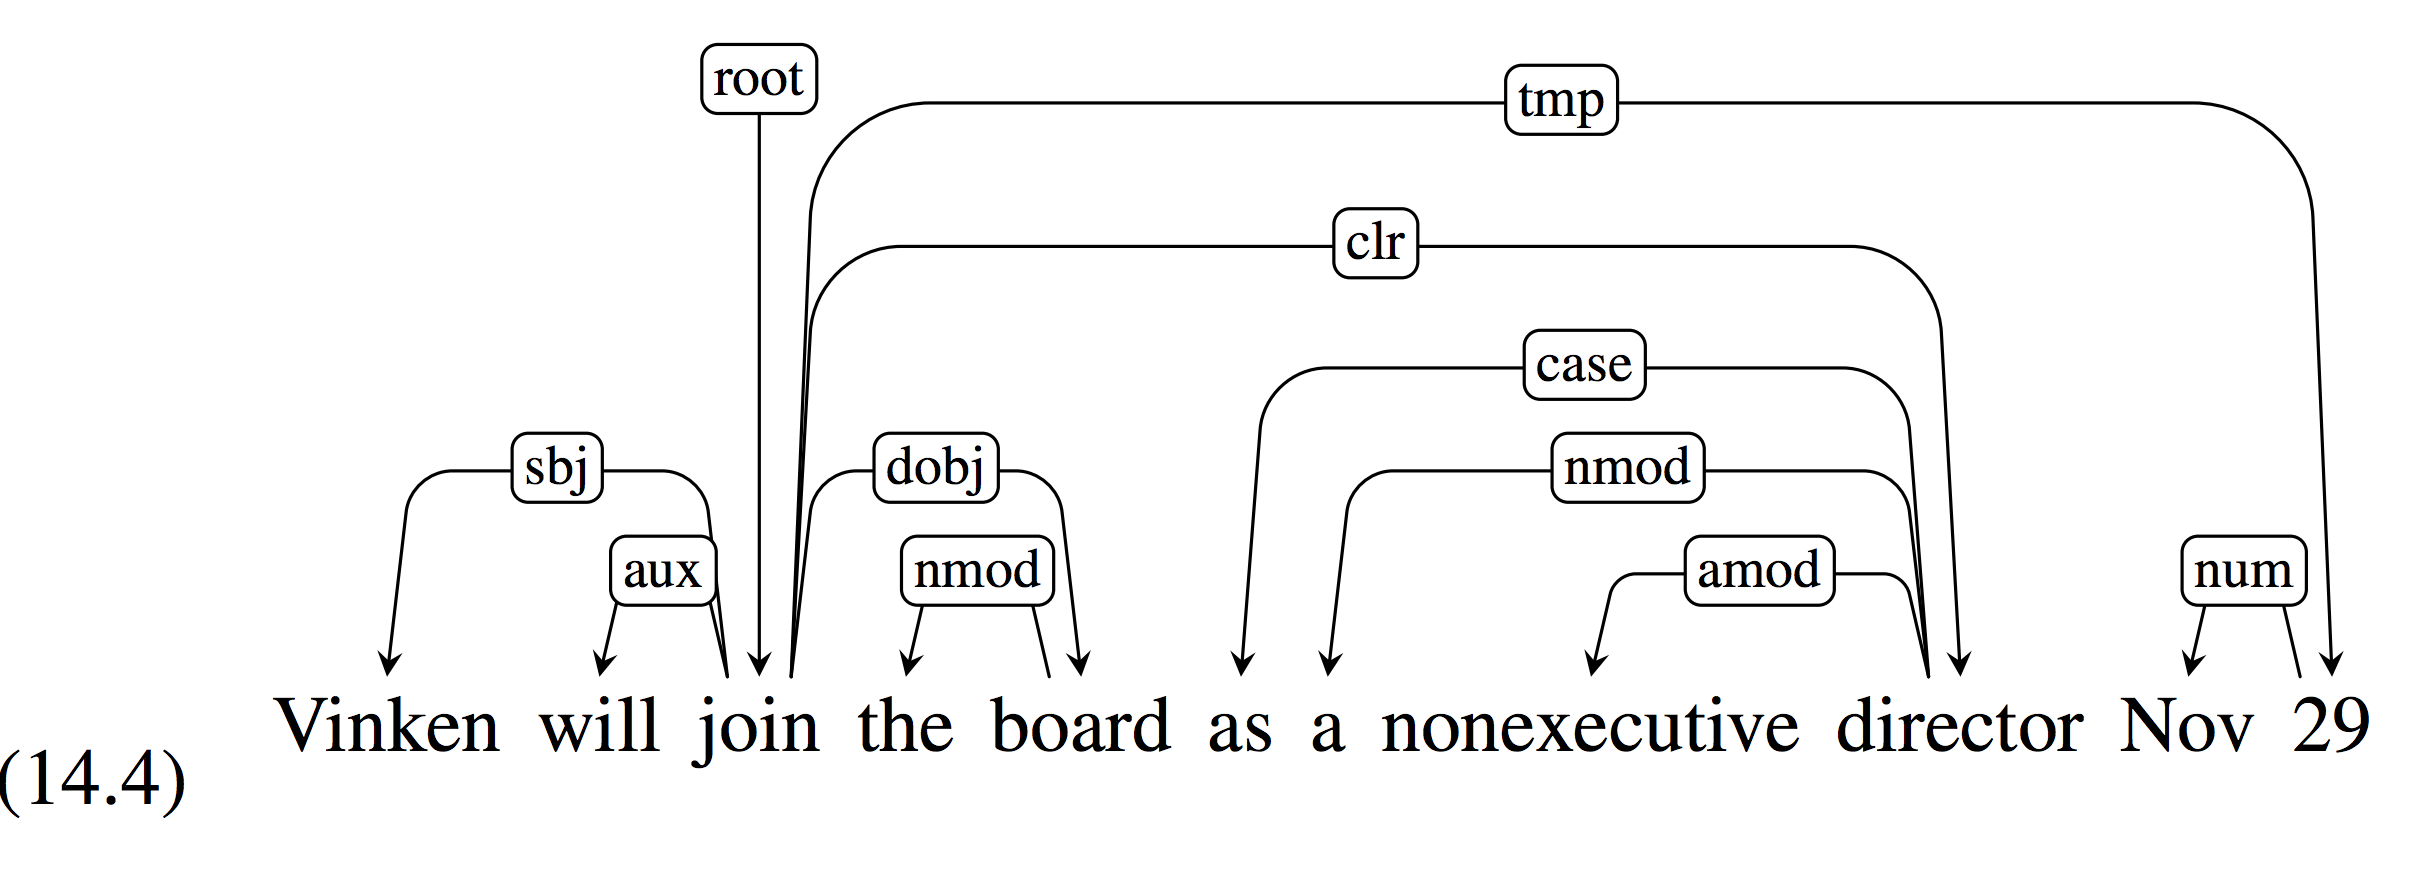
\includegraphics[width=\textwidth]{figures/dep1}
\end{frame}

\begin{frame}{Exercise: Constituent Structure \& Dependency Structure}

  How much wood would a woodchuck chuck if a woodchuck could chuck
  wood?

\end{frame}

\begin{frame}{English Resource Grammar}

  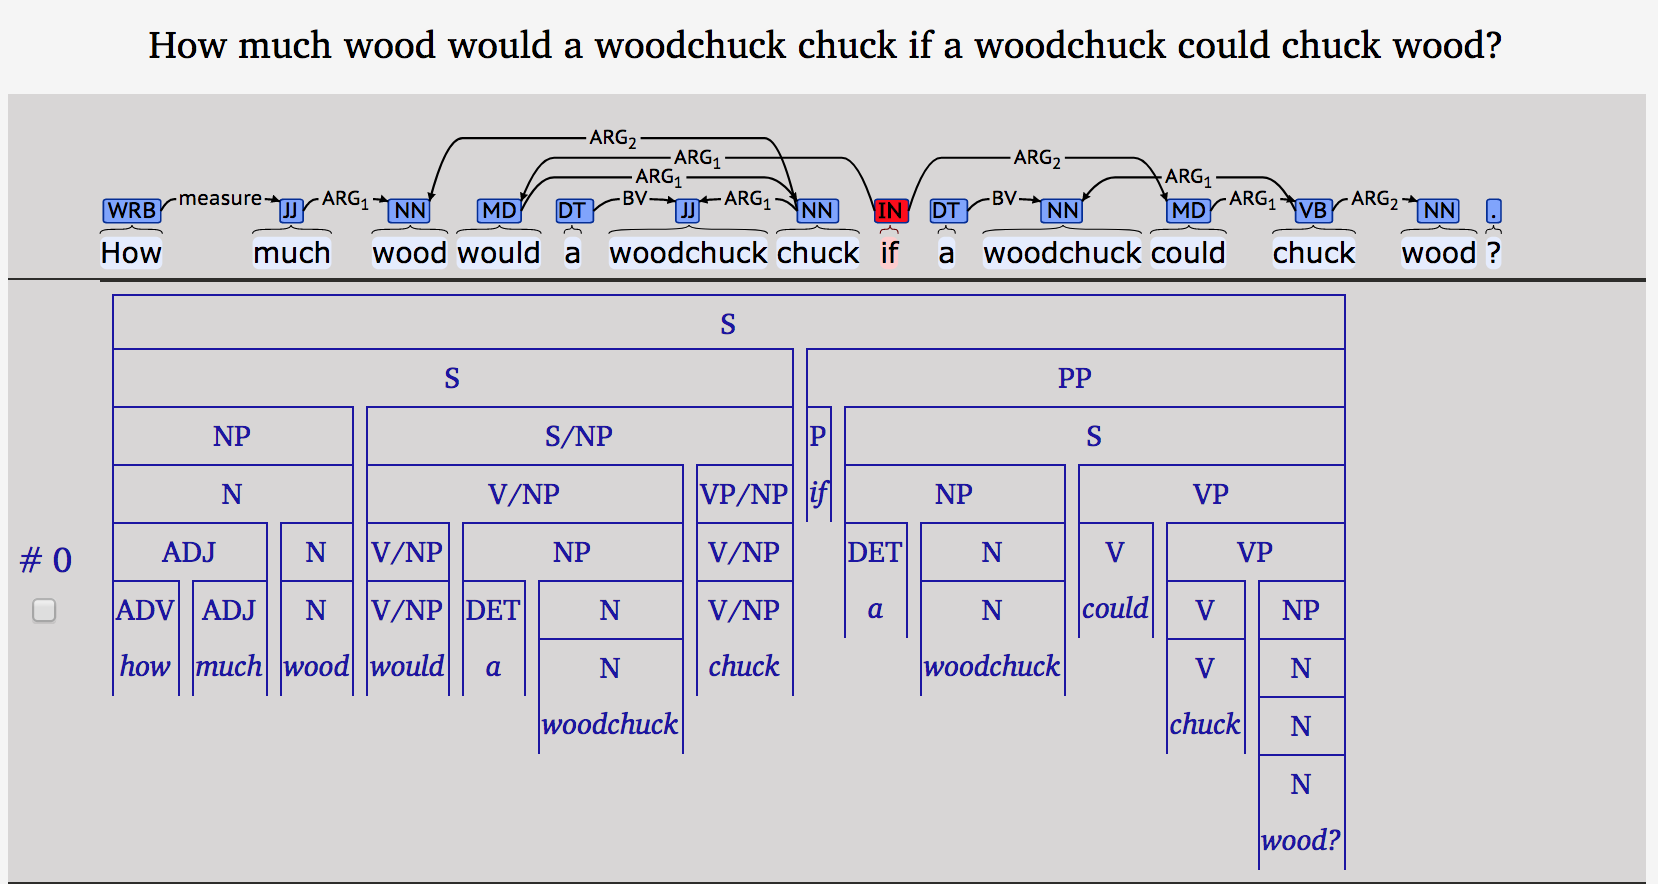
\includegraphics[width=\textwidth]{figures/woodchuck}

\end{frame}

\begin{frame}{Stanford Parser}

  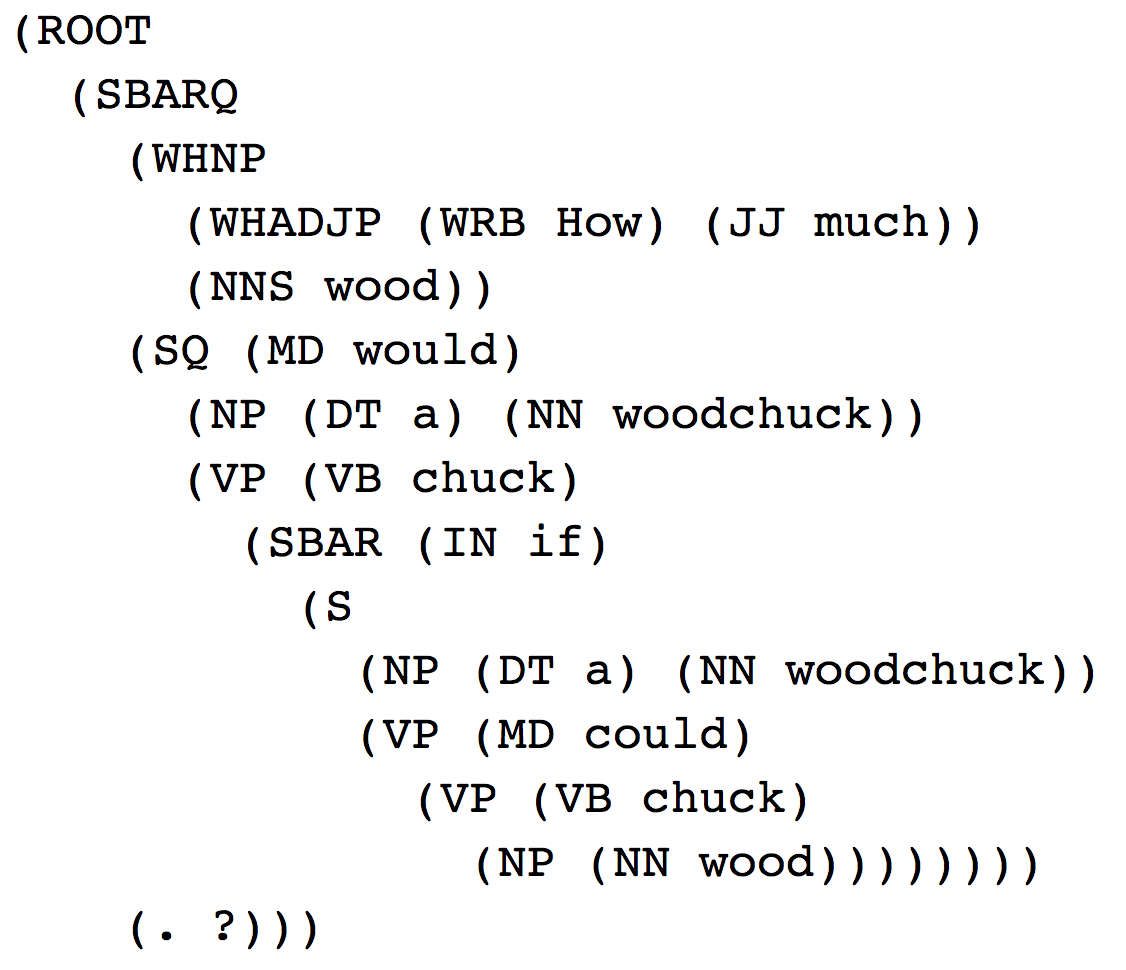
\includegraphics[width=\textwidth]{figures/stanford}

\end{frame}

\begin{frame}{When do we need structure?}
  \begin{itemize}
  \item When do we need constituent structure?
  \item When do we need dependency structure?
  \end{itemize} %
  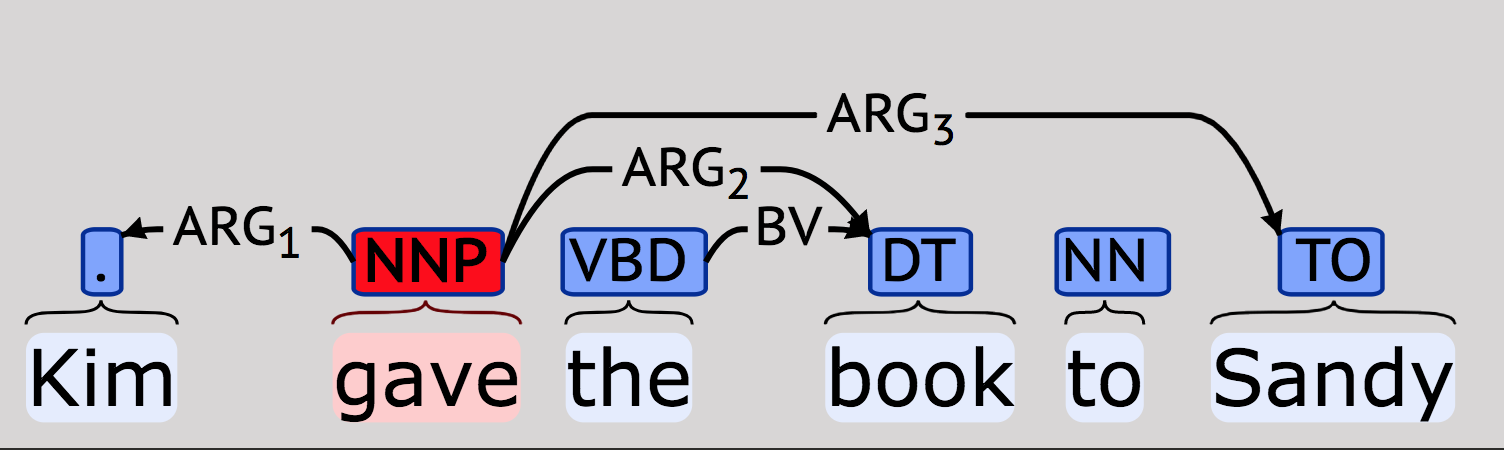
\includegraphics[width=0.4\textwidth]{figures/depend1} %
  % \begin{minipage}{0.5\textwidth}
  \begin{footnotesize}
\begin{forest}
  [S
  [NP [Kim]]
  [VP [V [gave]] [NP [D[the]] [N[book]]] [PP [P [to]] [NP [Sandy]]]]
  ]
\end{forest} 
\end{footnotesize}
\end{frame}

\begin{frame}{When do we need structure?}
  \begin{itemize}
  \item When do we need constituent structure?
    \begin{itemize}
    \item Structured language models (ASR, MT)
    \item Translation models (MT)
    \item Generation
    \item TTS: assigning intonation information
    \end{itemize}
  \item When do we need dependency structure?
    \begin{itemize}
    \item Information extraction (... QA, machine reading)
    \item Dialogue systems
    \item Sentiment analysis 
    \item Transfer-based MT
    \end{itemize}
  \end{itemize}
\end{frame}

\begin{frame}{Ambiguity}

  Parsing: Making explicit the structure that is inherent (implicit)
  in natural language strings

  \begin{itemize}
  \item How does it relate to the ambiguity issue?
  \item Suppose you have a parser. Does it help you with ambiguity?
  \end{itemize}
  
  \begin{minipage}{0.4\textwidth}
    \tiny
    \adjustbox{left=0.5\linewidth}{
      \begin{forest}
        [S
        [NP 
        [I]]
        [VP
        [saw]
        [NP [the] [astronomer]
        [PP [with the telescope,roof]]]
        ]
        ]
      \end{forest}
    }
  \end{minipage}
  \begin{minipage}{0.4\textwidth}
    \tiny
    \begin{forest}
      [S
      [NP 
      [I ]]
      [VP
      [saw]
      [NP [the] [astronomer]]
      [PP [with the telescope,roof]]
      ]
      ]
    \end{forest}
  \end{minipage}
\end{frame}

\begin{frame}{Ambiguity}

  Parsing: Making explicit structure that is inherent (implicit) in
  natural language strings

  \begin{itemize}
  \item How does it relate to the ambiguity issue?
  \item Suppose you have a parser. Does it help you with ambiguity?
    \begin{itemize}
    \item Depends on what you want:
    \item It helps {\bf expose} ambiguity
    \item ...but it does {\bf not} remove it
    \item parse ranking: choose one parse based on e.g.\ a language model
    \end{itemize}
  \end{itemize}
  
  \begin{minipage}{0.4\textwidth}
    \tiny
    \adjustbox{left=0.5\linewidth}{
      \begin{forest}
	[S
        [NP 
        [I]]
        [VP
        [saw]
        [NP [the] [astronomer]
        [PP [with the telescope,roof]]]
        ]
	]
      \end{forest}
    }
  \end{minipage}
  \begin{minipage}{0.4\textwidth}
    \tiny
    \begin{forest}
      [S
      [NP 
      [I ]]
      [VP
      [saw]
      [NP [the] [astronomer]]
      [PP [with the telescope,roof]]
      ]
      ]
    \end{forest}
  \end{minipage}
\end{frame}

\section{CFG}

\begin{frame}{The Chomsky hierarchy}
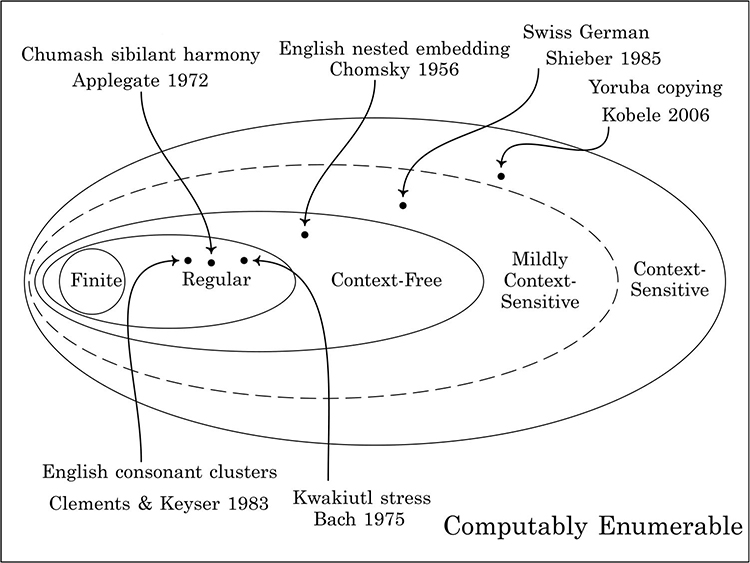
\includegraphics[width=\textwidth]{figures/language-hierarchy}
\end{frame}

\begin{frame}{Context Free Grammars}
  \begin{itemize}
  \item Context-Free Grammars generate Context-Free Languages
  \item CF languages fit into the Chomsky hierarchy between regular languages and context-sensitive languages
    \begin{itemize}
    \item All regular languages are also context free languages
    \item All sets of strings describable by FSAs can be described by a CFG
    \item But not vice versa 
    \end{itemize}
  \end{itemize}
\end{frame}

\begin{frame}{Context Free Grammars}

\begin{center}
NP $\rightarrow$ Det N
\vspace{1cm}

\begin{forest}
[NP [Det] [N]]
\end{forest}
\end{center}

\begin{itemize}
\item Represent constituent structure
\item Encode a sharp notion of grammaticality
  \begin{itemize}
  \item Compare to N-gram models
  \end{itemize}
\end{itemize}
\end{frame}

\begin{frame}{Grammaticality}

  \begin{itemize}
  \item What is a {\bf grammatical} sentence?
  \item What is an {\bf ungrammatical} sentence?
  \item Which sentences are grammatical?
    \begin{itemize}
    \item {\it I want to book a flight to Boston}
    \item {\it I want to booked a flight to Boston}
    \item {\it Colorless green ideas sleep furiously}
    \item {\it Twas brillig, and the slithy toves did gyre and gimble in the wabe}
    \end{itemize}
    \begin{itemize}
    \item ...from a CFG's point of view?
    \item ...from a probabilistic model point of view?
    \item ...from a human point of view?
    \end{itemize}
  \end{itemize}
\end{frame}

\begin{frame}{CFGs, informally}
  \begin{itemize}
  \item Consist of {\bf rules}, or {\bf productions}
    \begin{itemize}
    \item each expresses the ways that symbols of the language can be grouped and ordered 
    \end{itemize}
  \item ...and a {\bf lexicon} of words and symbols.
  \end{itemize}
  
NP $\rightarrow$ Det Nominal

NP  $\rightarrow$  ProperNoun

Nominal  $\rightarrow$  Noun $\vert$ Nominal Noun

Det $\rightarrow$ {\it a}

Det $\rightarrow$ {\it the}

Noun $\rightarrow$ {\it flight}
\end{frame}

\begin{frame}{CFGs, formally}
  \begin{itemize}
  \item A CFG is a 4-tuple: $<$ C, $\sum$, P, S $>$:
    \begin{itemize}
    \item C is the set of categories (aka non-terminals, e.g., \{ S,
      NP, VP, V, ...\} )
    \item $\sum$ is the vocabulary (aka terminals, e.g., \{ Kim, snow,
      adores, ... \})
    \item P is the set of rewrite rules, of the form:
      $\alpha \rightarrow \beta_1, \beta_2, ...,\beta_n$
    \item S (in C) is the start-symbol
    \item For each rule
      $\alpha \rightarrow \beta_1, \beta_2, ...,\beta_n$ in P,
      $\alpha$ is drawn from C and each $\beta$ is drawn from C or
      $\sum$
    \end{itemize}
\end{itemize}
\end{frame}

\begin{frame}{Parsing and Generation}
  \begin{itemize}
  \item ...familiar dualism
    \begin{itemize}
    \item recall FSTs
    \end{itemize}
  \item {\bf Parsing}: assigning a structure to a string
  \item {\bf Generation}: using rules to write strings
  \item {\bf Derivation}: Arriving from a string to a structure (or vice versa) by applying a series of rules
  \end{itemize}
\end{frame}

\begin{frame}{The Start symbol}
  \begin{itemize}
  \item Is needed for us to know where to start (or finish), to get a well-formed structure
    \begin{itemize}
    \item Would we want to start deriving from VP?
      \begin{itemize}
      \item maybe! depends on the situation
      \end{itemize}
    \end{itemize}
  \item When denoted {\it S}, is easy to think of as referring to ``sentence'', but it need not be the case
  \item It really refers to ``Start'', not ``sentence''.
  \end{itemize}
\end{frame}

\begin{frame}{CFG Example}
  \begin{itemize}
  \item {\it Book my flight. Do you know the number? He gave me the
      number. He served my dinner.}
  \item Using the following lexicon, write rules that will generate
    (at least) these sentences, and assign them plausible structures.
    \begin{itemize}
    \item Aux = \{do, does\}
    \item V = \{book, know, gave, serve, served\}
    \item N = \{flight, number, dinner, you, me, he\} 
    \item Det = \{my, the\}
    \end{itemize}
\end{itemize}
\end{frame}

\begin{frame}{CFG Example, candidate grammar}
  \begin{itemize}
  \item {\it Book my flight. Do you know the number? He gave me the number. He served my dinner.}
    \begin{itemize}
    \item Aux = \{do, does\}
    \item V = \{book, know, gave, serve, served\}
    \item N = \{flight, number, dinner, you, me, he\} 
    \item Det = \{my, the\}
    \item S $\rightarrow$ NP VP $\vert$ VP $\vert$ Aux S
    \item NP $\rightarrow$ Det N
    \item VP $\rightarrow$ V NP (NP)
    \end{itemize}
  \end{itemize}
  What is missing? How to fix it?
\end{frame}

\begin{frame}{CFG Example, candidate grammar}
  \begin{itemize}
  \item {\it Book my flight. Do you know the number? He gave me the number. He served my dinner.}
    \begin{itemize}
    \item Aux = \{do, does\}
    \item V = \{book, know, gave, serve, served\}
    \item N = \{flight, number, dinner\} 
    \item PRO = \{me, you, he\}
    \item Det = \{my, the\}
    \item S $\rightarrow$ NP VP $\vert$ VP $\vert$ Aux S
    \item NP $\rightarrow$ Det N $\vert$ PRO
    \item VP $\rightarrow$ V NP (NP)
    \end{itemize}
  \end{itemize}
  
  Better?
\end{frame}

%\begin{frame}
%\frametitle{CFG Example}
%\begin{itemize}
%\item {\it Book my flight. Do you know the number? He gave me the number. He served my dinner.}
%\begin{itemize}
%\item Aux = \{do, does\}
%\item V = \{book, know, gave, serve, served\}
%\item N = \{flight, number, dinner\} 
%\item PRO = \{me, you, he\}
%\item Det = \{my, the\}
%\item S $\rightarrow$ NP VP $\vert$ VP $\vert$ Aux S
%\item NP $\rightarrow$ Det N $\vert$ PRO
%\item VP $\rightarrow$ V NP (NP)
%\end{itemize}
%\end{itemize}
%
%{\it Does the flight serve dinner?} (Problem?)
%
%\end{frame}

\begin{frame}{CFG Example}
  \begin{itemize}
  \item {\it Book my flight. Do you know the number? He gave me the number. He served my dinner.}
    \begin{itemize}
    \item Aux = \{do, does\}
    \item V = \{book, know, gave, serve, served\}
    \item N = \{flight, number, dinner\} 
    \item PRO = \{me, you, he\}
    \item Det = \{my, the\}
    \item S $\rightarrow$ NP VP $\vert$ VP $\vert$ Aux S
    \item NP $\rightarrow$ Det N $\vert$ PRO
    \item VP $\rightarrow$ V NP (NP)
    \end{itemize}
  \end{itemize}
  
  {\it *He serve my dinner} (Problem?)
\end{frame}

\begin{frame}{CFG Example}
  \begin{itemize}
  \item {\it Book my flight. Do you know the number? He gave me the number. He served my dinner.}
    \begin{itemize}
    \item Aux = \{do, does\}
    \item V = \{book, know, gave, serve, served, {\bf serves}\}
    \item N = \{flight, number, dinner\} 
    \item PRO = \{me, you, he\}
    \item Det = \{my, the\}
    \item S $\rightarrow$ NP VP $\vert$ VP $\vert$ Aux S
    \item NP $\rightarrow$ Det N $\vert$ PRO
    \item VP $\rightarrow$ V NP (NP)
    \end{itemize}
  \end{itemize}
  {\it *Does this flight serves you dinner} (Problem?)
\end{frame}

\begin{frame}{CFG Example}
  \begin{itemize}
  \item {\it Book my flight. Do you know the number? He gave me the number. He served my dinner.}
    \begin{itemize}
    \item AuxSG = \{does\}
    \item AuxPL = \{do\}
    \item V-PL = \{book, know, gave, serve, served\}
    \item V-SG = \{books, knows, gave, serves, served\}
    \item N-SG = \{flight, number, dinner\} 
    \item N-PL = \{flights, numbers, dinners\} 
    \item PRO-SG = \{me, you, he\}
    \item PRO-PL = \{you\}
    \item Det = \{my, the\}
    \item S $\rightarrow$ NP VP $\vert$ VP $\vert$ Aux S
    \item NP-SG $\rightarrow$ Det N-SG $\vert$ PRO
    \item NP-SG $\rightarrow$ Det N-PL $\vert$ PRO
    \item VP $\rightarrow$ V NP (NP)
    \end{itemize}
  \end{itemize}
  
  Problem?
\end{frame}


\begin{frame}{Limitations of CFGs}

  {\it The cat chases the mouse} vs. {\it *The cat chase the mouse}
  
  \begin{itemize}
  \item Can we model agreement?
    \begin{itemize}
    \item Sure. But the grammar will quickly become rather huge and inelegant!
      \begin{itemize}
      \item ...will need duplicate rules whenever 3rd person singular and plural are involved
      \item ...what about languages with lots of various inflections?
      \end{itemize}
    \end{itemize}
  \item what about relating passive and interrogative sentences to
    their declarative counterparts?
  \item how many subtypes of verbs will we need?
    \begin{itemize}
    \item For each {\bf subcategorization frame}, we will need to
      duplicate all the appropriate rules
    \end{itemize}
  \end{itemize}
\end{frame}

\begin{frame}
\frametitle{What about heads?}

\begin{itemize}
\item A {\bf head} in syntactic theory is an item that is the most important in the phrase
\item Essential for dependency parsing and probabilistic parsing
\item Can we augment CFG with heads?
\end{itemize}
\end{frame}

\begin{frame}{What about heads?}

  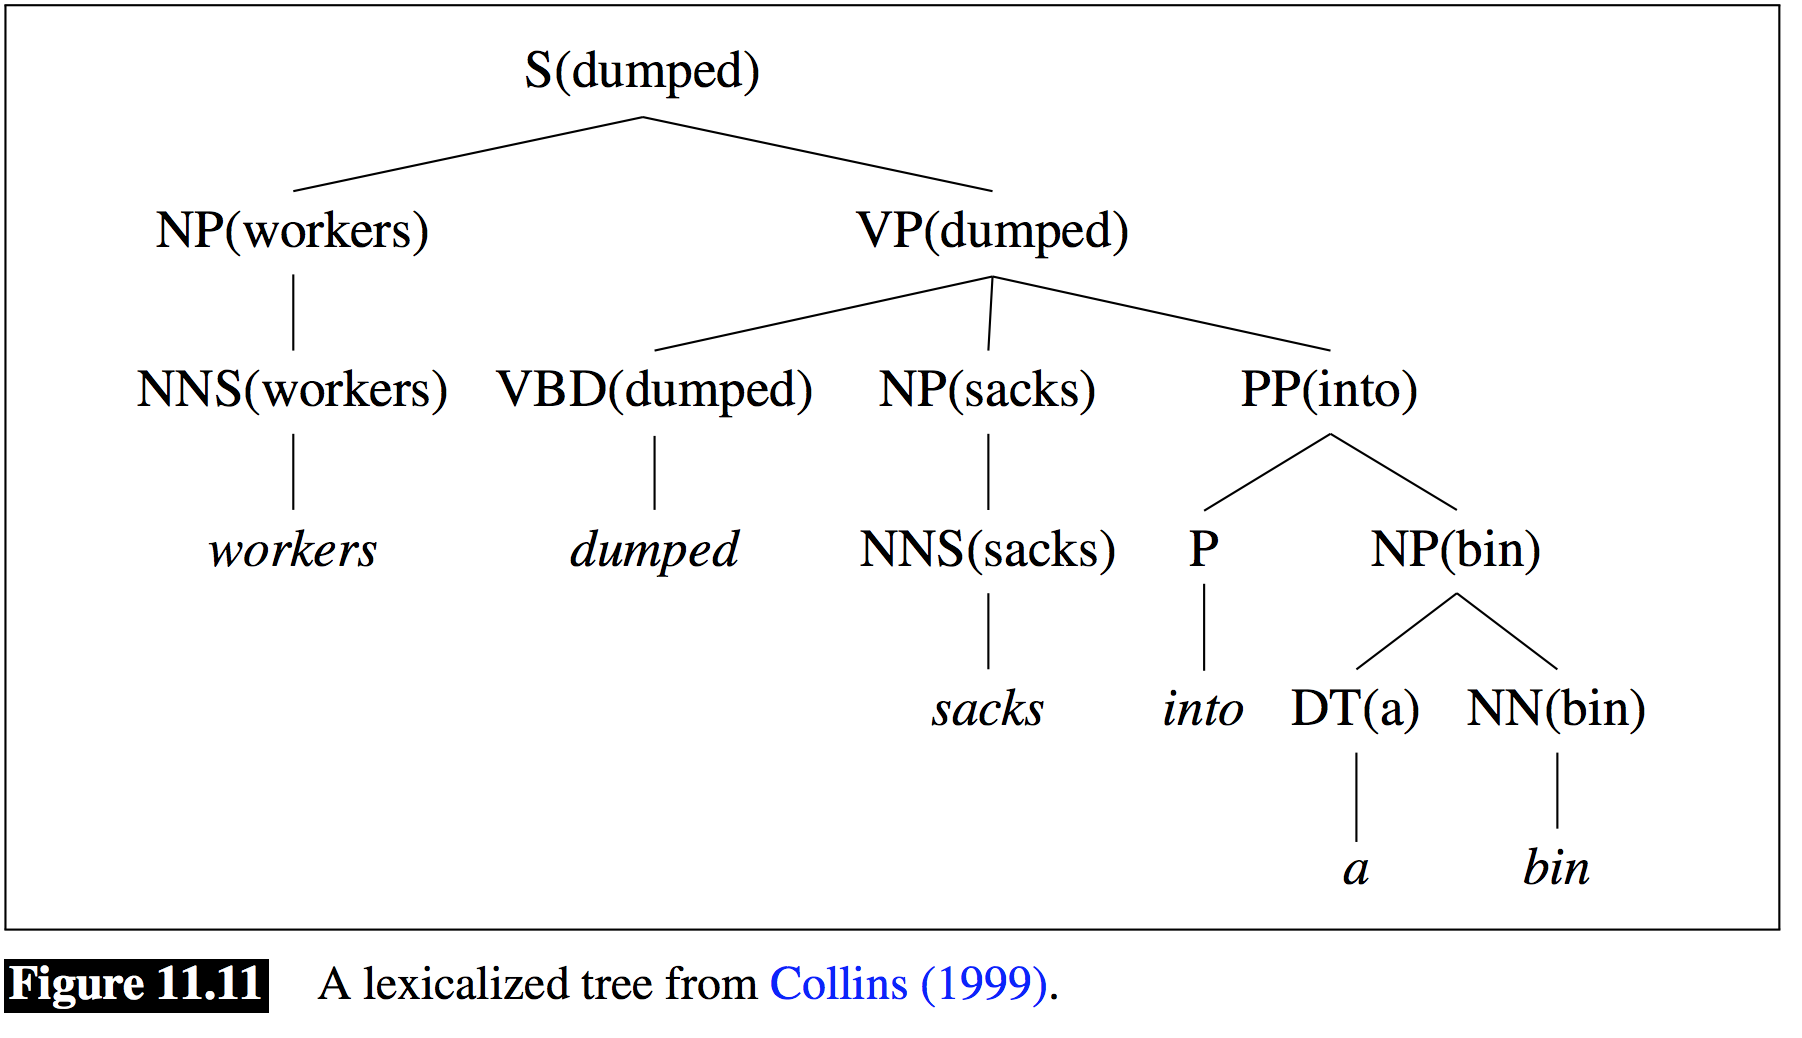
\includegraphics[width=\textwidth]{figures/heads}

\end{frame}

\begin{frame}{Parsing algorithms and grammars}
  \begin{itemize}
  \item A grammar is typically {\bf input} to a parser
  \item (e.g. we've been parsing by hand, using CFGs)
  \item Grammars can be engineered or learned statistically from corpora
    \begin{itemize}
    \item Both approaches have pros and cons
    \item In particular, engineered grammars have higher {\bf
        precision} while statistically-learned grammars have higher
      {\bf recall}
    \item why?
    \end{itemize}
  \end{itemize}
\end{frame}

\section{Evaluation}

\begin{frame}{Evaluating parsing}
  \begin{itemize}
  \item How would you do extrinsic evaluation of a parsing system?
  \item How would you do intrinsic evaluation?
    \begin{itemize}
    \item Gold standard data?
    \item Metrics?
    \end{itemize}
  \end{itemize}
\end{frame}

\begin{frame}{Gold standard}
  \begin{itemize}
  \item What would a gold standard look like?
  \end{itemize}
\end{frame}

\begin{frame}{Gold standard}
  \begin{itemize}
  \item A corpus of string-to-structure mappings
  \item Is this different from a corpus of hand-written digit to actual digit mappings?
  \item From a corpus of string-to-POS sequence mappings?
  \end{itemize}
\end{frame}

\begin{frame}{Gold standard}
  \begin{itemize}
  \item A corpus of string-to-structure mappings
  \item But: there's no ground truth in trees!
  \item Semantic dependencies might be easier to get cross-framework
    agreement on, but even there it's non-trivial
  \item The Penn Treebank (Marcus et al 1993) was originally conceived
    of as a target for cross-framework parser evaluation
  \item For project-internal/regression testing, grammar-based
    treebanking is effective for creating (g)old-standard data
  \end{itemize}
\end{frame}

\begin{frame}{Metrics: Parseval}
  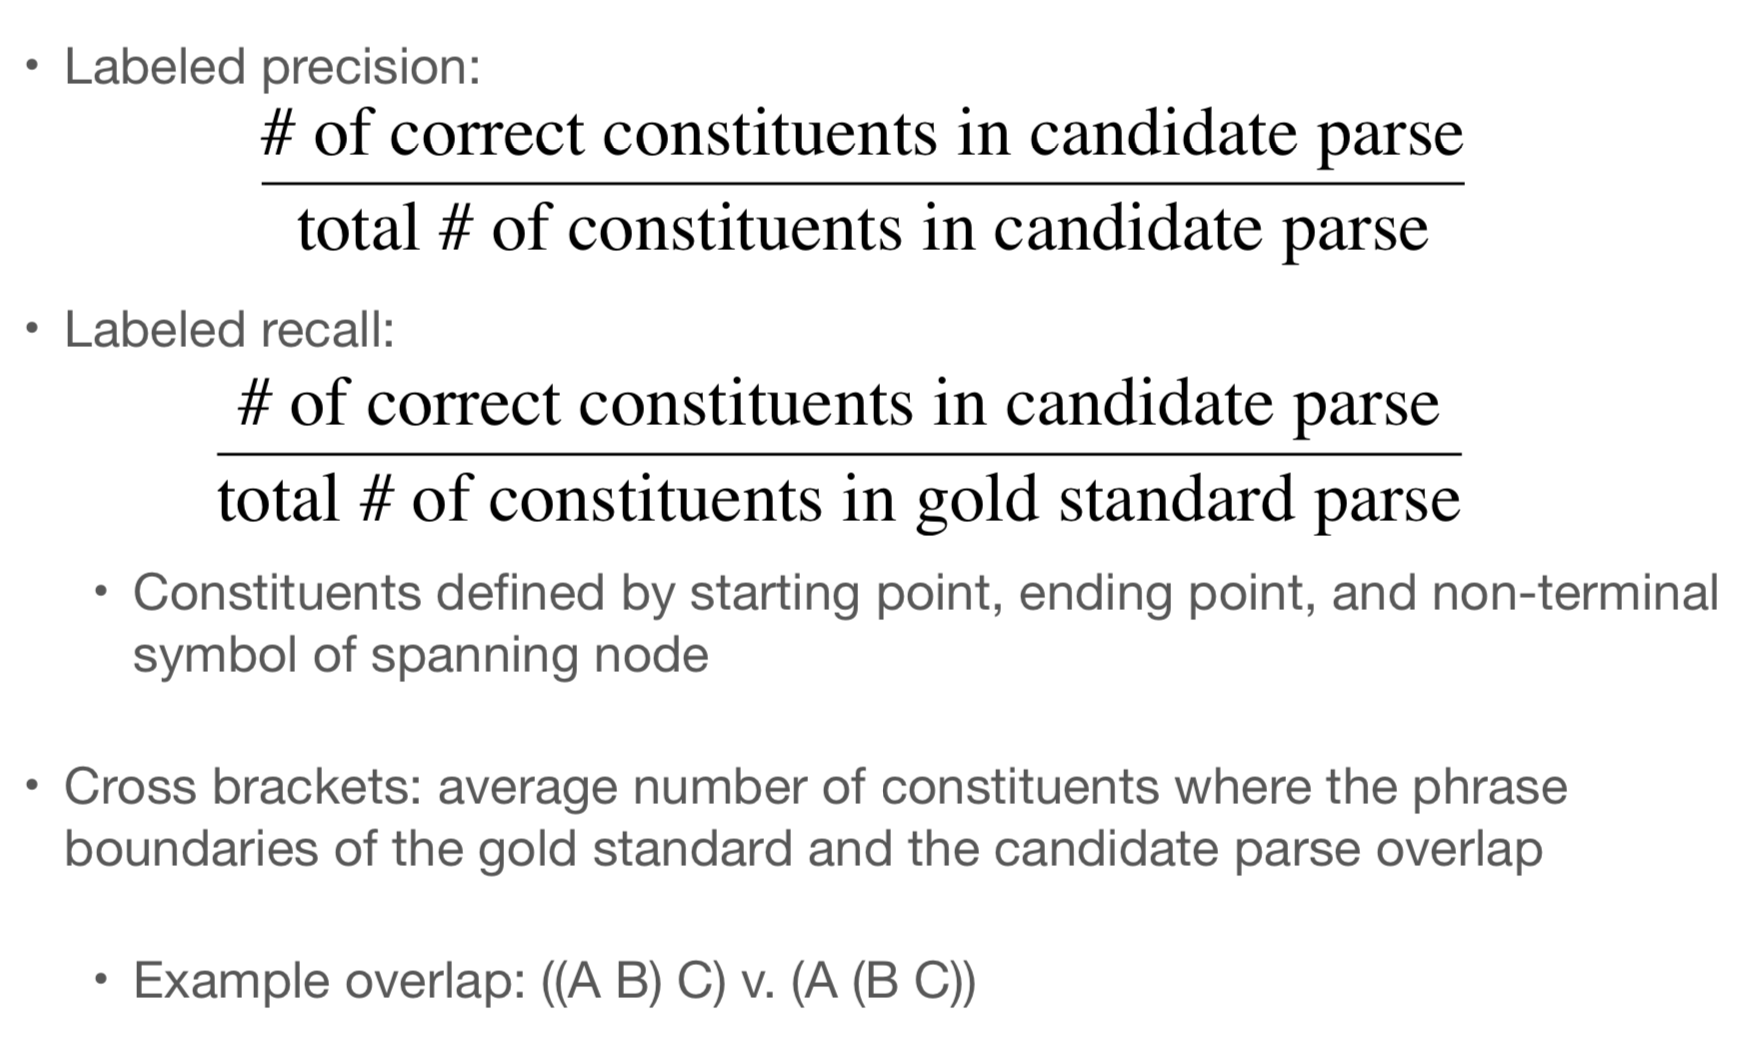
\includegraphics[width=\textwidth]{figures/parseval}
\end{frame}

\section{Treebanking}

\begin{frame}{Treebanking}

  \begin{itemize}
  \item A {\bf treebank} is a syntactically annotated corpus
  \end{itemize}

  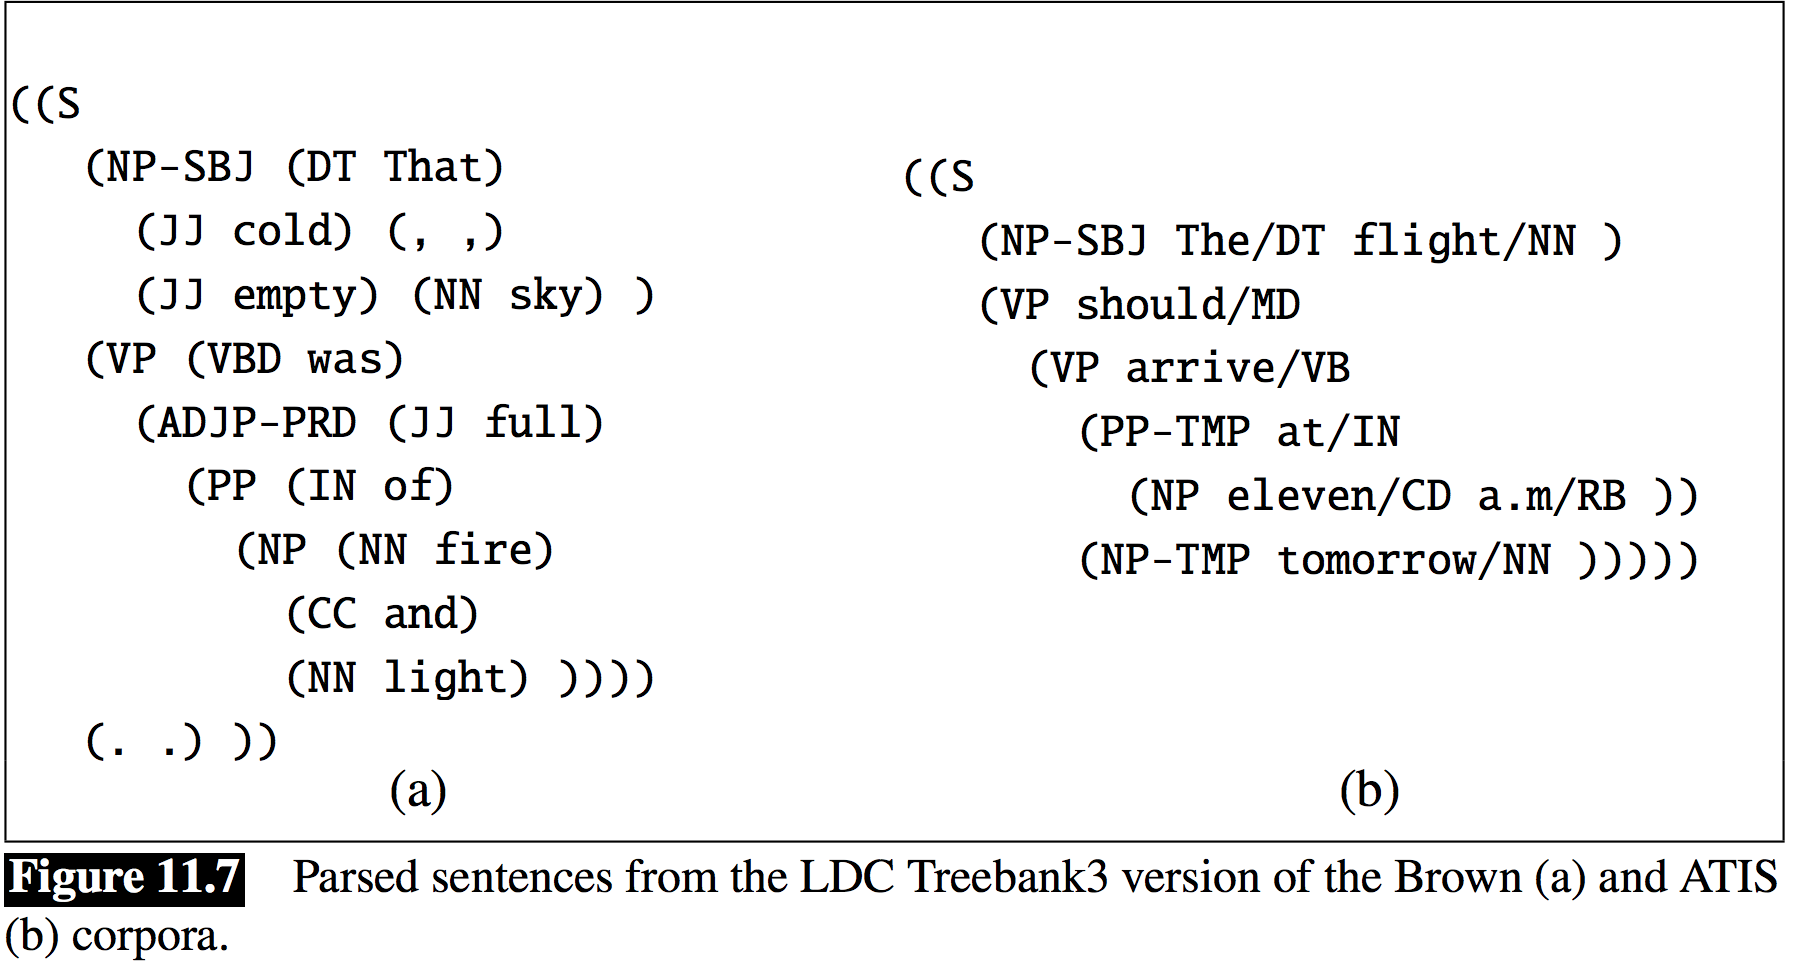
\includegraphics[width=\textwidth]{figures/treebank}
\end{frame}

\begin{frame}{Tree visualization}

\begin{forest}
[S
  [NP-SBJ
     [DT [the]]
     [NN [flight]]
  ]
  [VP
     [MD [should]]
     [VP
         [VB [arrive]]
         [PP-TMP
             [IN [at]]
             [NP [CD [eleven]] [RB [a.m.]] ]
         ]
         [NP-TMP [NN [tomorrow]] ]
     ]
  ]
]
\end{forest}
\end{frame}

\begin{frame}{Treebanks as grammars}
\begin{itemize}
\item How to turn a treebank into a grammar?
  \begin{itemize}
  \item Extract the rewrite rules
  \item We could also count how many times we saw which production
    \begin{itemize}
    \item Anything useful we could do with that?
    \end{itemize}
  \end{itemize}
\end{itemize}
\end{frame}

\begin{frame}{Treebanks as grammars}
  \begin{itemize}
  \item How to turn a treebank into a grammar?
    \begin{itemize}
    \item Extract the rewrite rules
    \item Exercise: extract the rules from the sample treebank sentences in the previous slide
    \end{itemize}
  \end{itemize}
\end{frame}


\begin{frame}{Treebanks as grammars}
\begin{itemize}
\item How to turn a treebank into a grammar?
  \begin{itemize}
  \item Extract the rewrite rules
  \item We could also count how many times we saw which production (See \href{https://youtu.be/HSAUqdDnYEU})
    \begin{itemize}
    \item Anything useful we could do with that?
    \item Statistical parsing! 
    \end{itemize}
  \end{itemize}
\end{itemize}
\end{frame}

\begin{frame}{Dependency Formalisms and Treebanks}
  \begin{itemize}
  \item The Penn Treebank (Marcus et al., 1993)
  \item Universal Dependencies (Nivre et al., 2016)
  \end{itemize}
  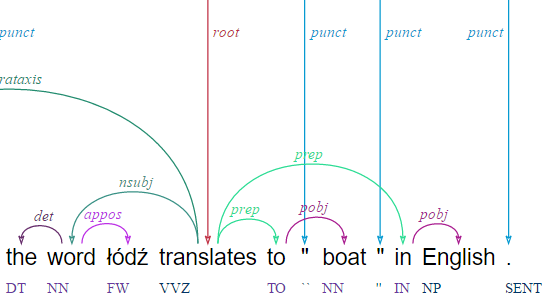
\includegraphics[height=0.6\textheight]{figures/ud}
\end{frame}

\begin{frame}{Dependency Treebank}
  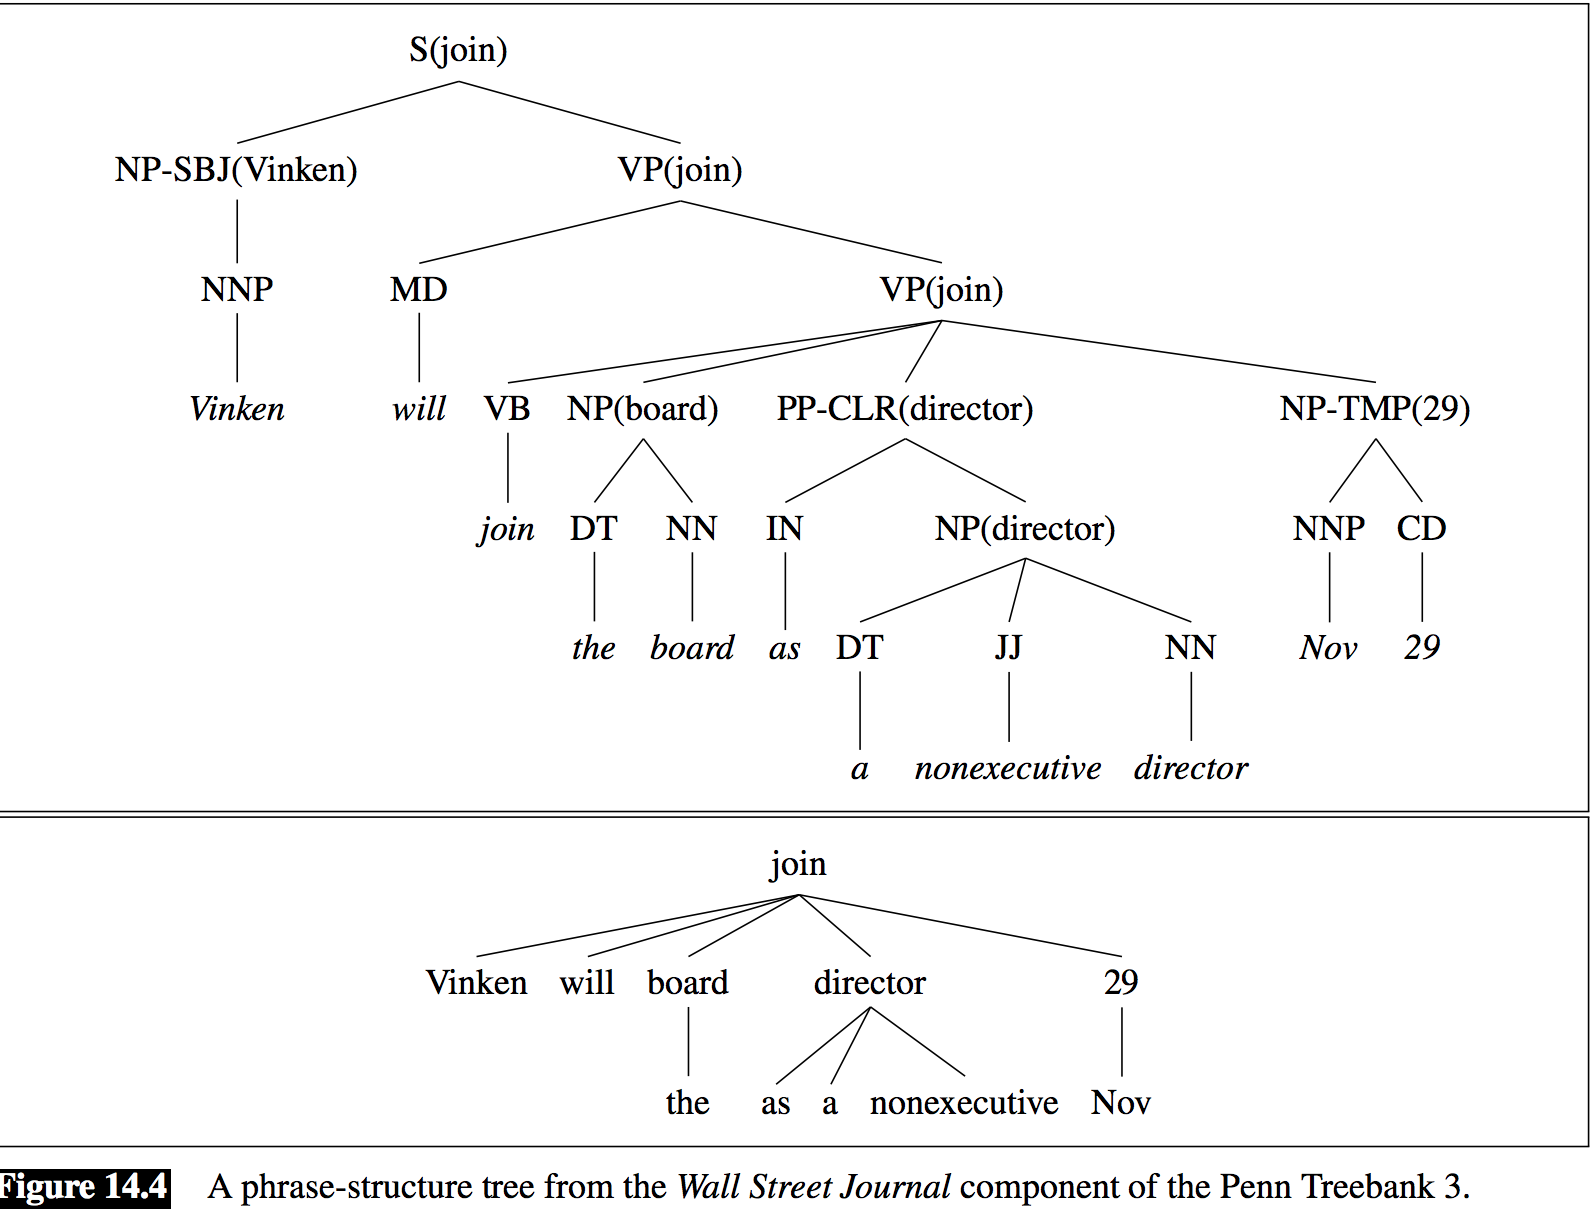
\includegraphics[width=\textwidth]{figures/dep2}
\end{frame}

\section{Summary}

\begin{frame}{What you need to know}
  \begin{itemize}
  \item Parsing, grammar, grammaticality definitions
  \item Bracket and tree notation
  \item CFGs: informal definition, production, derivation
  \item Treebanks (what they are)
  \end{itemize}
\end{frame}

\end{document}

%%% Local Variables:
%%% mode: latex
%%% TeX-master: t
%%% End:
